% !TeX root = ../main.tex

% =================== 文獻探討 =================== %
\section{文獻探討}

這是 \textbf{粗體},這是 \underline{底線},這是 \textit{斜體}.

% ------------------- 小標題 -------------------- %
\subsection{小標題}

論文引用測試 \cite{Rowe:2005:ASR};引用多篇測試 \cite{Rowe:2005:ASR,vinet1989universal}。
圖片測試,圖 \ref{figure:fig1}。

% ------------------- 小小標題 ------------------- %
\subsubsection{小小標題}

\begin{figure}[htbp]
    \centering
    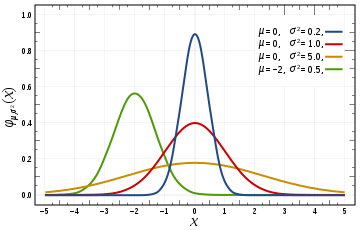
\includegraphics[width=0.5\textwidth]{figures/gambar.png}
    \caption{範例圖片}
    \label{figure:fig1}
\end{figure}

% 插入背景為白色的gamber.png
\begin{figure}[htbp]
    \centering
    \colorbox{white}{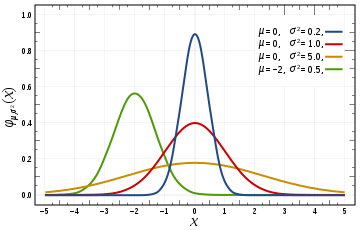
\includegraphics[width=0.5\textwidth]{figures/gambar.png}}
    \caption{範例白底圖片}
    \label{figure:fig2}
\end{figure}


% ------------------- 列點範例 ------------------ %
\subsection{列點範例}

\begin{itemize}
    \item 個別項目以黑點表示,稱為項目符號。
    \item 項目中的文字可以是任意長度。
\end{itemize}

\begin{enumerate}
    \item 這是我們清單中的第一個項目。
    \item 隨著每個新增的項目,清單編號會增加。
\end{enumerate}

% ------------------- 子圖範例 ------------------ %
\clearpage
\subsection{子圖範例}

\begin{figure}[htbp]
    \centering
    \begin{subfigure}[b]{0.3\textwidth}
        \centering
        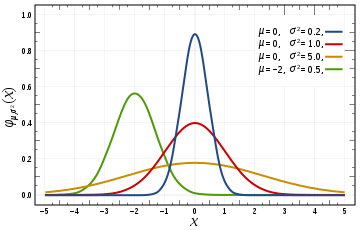
\includegraphics[width=\textwidth]{figures/gambar.png}
        \caption{$y=x$}
        \label{fig:y equals x}
    \end{subfigure}
    \hfill
    \begin{subfigure}[b]{0.3\textwidth}
        \centering
        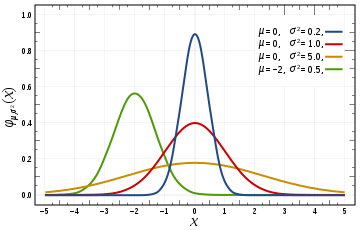
\includegraphics[width=\textwidth]{figures/gambar.png}
        \caption{$y=3\sin x$}
        \label{fig:three sin x}
    \end{subfigure}
    \hfill
    \begin{subfigure}[b]{0.3\textwidth}
        \centering
        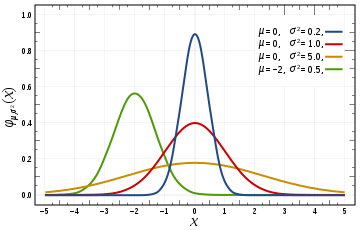
\includegraphics[width=\textwidth]{figures/gambar.png}
        \caption{$y=5/x$}
        \label{fig:five over x}
    \end{subfigure}
       \caption{三子圖範例}
       \label{fig:three graphs}
\end{figure}

\begin{figure}[htbp]
    \centering
    \begin{subfigure}{0.4\textwidth}
        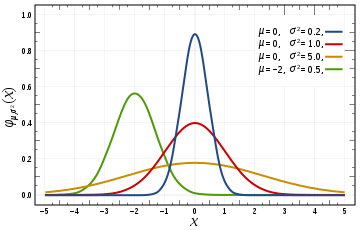
\includegraphics[width=\textwidth]{figures/gambar.png}
        \caption{Firts subfigure.}
        \label{fig:first}
    \end{subfigure}
    \hfill
    \begin{subfigure}{0.4\textwidth}
        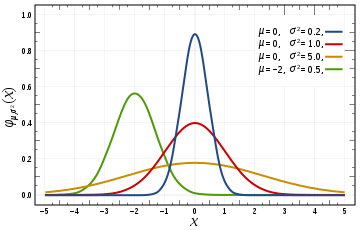
\includegraphics[width=\textwidth]{figures/gambar.png}
        \caption{Second subfigure.}
        \label{fig:second}
    \end{subfigure}
    \hfill
    \begin{subfigure}{0.4\textwidth}
        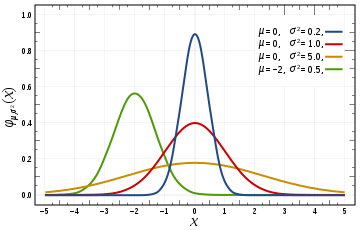
\includegraphics[width=\textwidth]{figures/gambar.png}
        \caption{Third subfigure.}
        \label{fig:third}
    \end{subfigure}
    \hfill
    \begin{subfigure}{0.4\textwidth}
        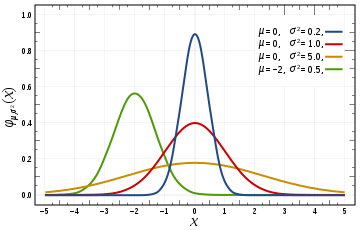
\includegraphics[width=\textwidth]{figures/gambar.png}
        \caption{Third subfigure.}
        \label{fig:fourth}
    \end{subfigure}
            
    \caption{四子圖範例}
    \label{fig:four graphs}
\end{figure}
